\documentclass[tikz, border=10pt]{standalone}
\usepackage{amsmath}
\usepackage{siunitx}

\begin{document}
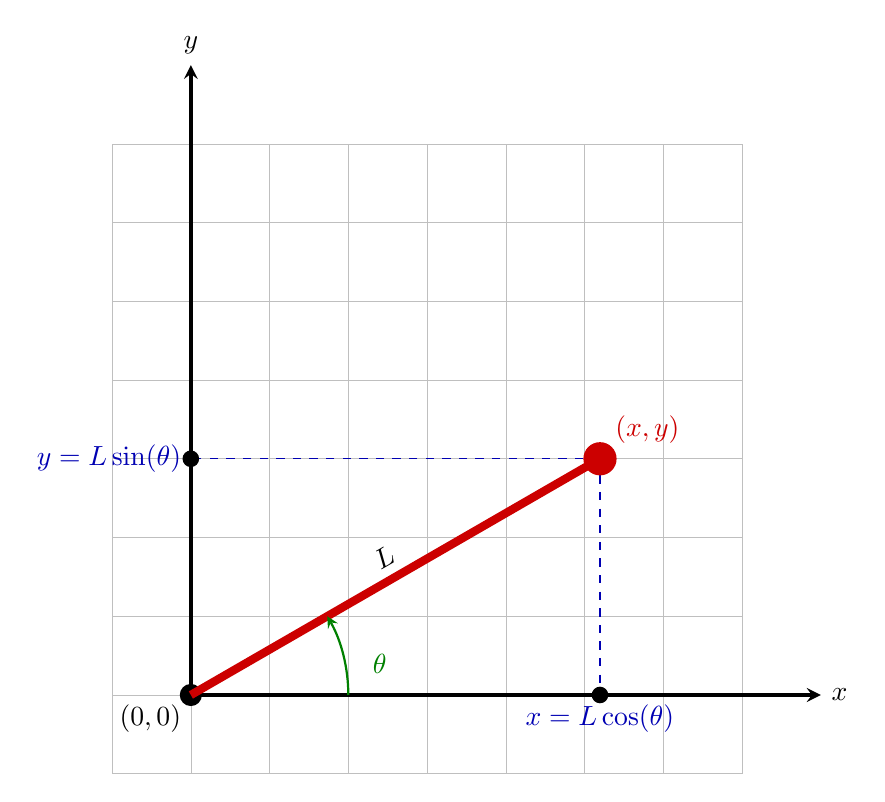
\begin{tikzpicture}[scale=2, >=stealth]

    % --- Configuration ---
    \def\L{3} % Length of the link
    \def\thetaValue{30} % Angle in degrees
    \pgfmathsetmacro{\xCoord}{\L*cos(\thetaValue)}
    \pgfmathsetmacro{\yCoord}{\L*sin(\thetaValue)}

    % --- Grid and Axes ---
    \draw[help lines, step=0.5, very thin, gray!50] (-0.5,-0.5) grid (3.5, 3.5);

    % Draw the main axes
    \draw[->, very thick] (0, 0) -- (4, 0) node[right] {$x$};
    \draw[->, very thick] (0, 0) -- (0, 4) node[above] {$y$};

    % Origin
    \fill (0, 0) circle (2pt) node[below left] {$(0,0)$};

    % --- Robot Arm Link ---
    \draw[line width=3pt, red!80!black] (0, 0) -- (\xCoord, \yCoord) node[midway, above, sloped, black] {$L$};

    % --- Projections (Dashed Lines) ---
    % Projection to x-axis
    \draw[dashed, blue!70!black] (\xCoord, \yCoord) -- (\xCoord, 0) node[below] {$x = L \cos(\theta)$};
    \fill (\xCoord, 0) circle (1.5pt);

    % Projection to y-axis
    \draw[dashed, blue!70!black] (\xCoord, \yCoord) -- (0, \yCoord) node[left] {$y = L \sin(\theta)$};
    \fill (0, \yCoord) circle (1.5pt);

    % Tip of the arm
    \fill[red!80!black] (\xCoord, \yCoord) circle (3pt) node[above right, xshift=2pt, yshift=2pt] {$(x, y)$};

    % --- Angle Annotation ---
    \draw[->, thick, green!50!black] (1, 0) arc (0:\thetaValue:1);
    \node at (1.2, 0.2) [green!50!black] {$\theta$};

    % --- Coordinate Labels (Optional - for clarity) ---
    % \node at (\xCoord/2, -0.3) {}; % Already labeled below x-axis
    % \node at (-0.4, \yCoord/2) {}; % Already labeled left of y-axis

\end{tikzpicture}
\end{document}